% Options for packages loaded elsewhere
\PassOptionsToPackage{unicode}{hyperref}
\PassOptionsToPackage{hyphens}{url}
%
\documentclass[
  ignorenonframetext,
]{beamer}
\usepackage{pgfpages}
\setbeamertemplate{caption}[numbered]
\setbeamertemplate{caption label separator}{: }
\setbeamercolor{caption name}{fg=normal text.fg}
\beamertemplatenavigationsymbolsempty
% Prevent slide breaks in the middle of a paragraph
\widowpenalties 1 10000
\raggedbottom
\setbeamertemplate{part page}{
  \centering
  \begin{beamercolorbox}[sep=16pt,center]{part title}
    \usebeamerfont{part title}\insertpart\par
  \end{beamercolorbox}
}
\setbeamertemplate{section page}{
  \centering
  \begin{beamercolorbox}[sep=12pt,center]{part title}
    \usebeamerfont{section title}\insertsection\par
  \end{beamercolorbox}
}
\setbeamertemplate{subsection page}{
  \centering
  \begin{beamercolorbox}[sep=8pt,center]{part title}
    \usebeamerfont{subsection title}\insertsubsection\par
  \end{beamercolorbox}
}
\AtBeginPart{
  \frame{\partpage}
}
\AtBeginSection{
  \ifbibliography
  \else
    \frame{\sectionpage}
  \fi
}
\AtBeginSubsection{
  \frame{\subsectionpage}
}
\usepackage{amsmath,amssymb}
\usepackage{iftex}
\ifPDFTeX
  \usepackage[T1]{fontenc}
  \usepackage[utf8]{inputenc}
  \usepackage{textcomp} % provide euro and other symbols
\else % if luatex or xetex
  \usepackage{unicode-math} % this also loads fontspec
  \defaultfontfeatures{Scale=MatchLowercase}
  \defaultfontfeatures[\rmfamily]{Ligatures=TeX,Scale=1}
\fi
\usepackage{lmodern}
\ifPDFTeX\else
  % xetex/luatex font selection
\fi
% Use upquote if available, for straight quotes in verbatim environments
\IfFileExists{upquote.sty}{\usepackage{upquote}}{}
\IfFileExists{microtype.sty}{% use microtype if available
  \usepackage[]{microtype}
  \UseMicrotypeSet[protrusion]{basicmath} % disable protrusion for tt fonts
}{}
\makeatletter
\@ifundefined{KOMAClassName}{% if non-KOMA class
  \IfFileExists{parskip.sty}{%
    \usepackage{parskip}
  }{% else
    \setlength{\parindent}{0pt}
    \setlength{\parskip}{6pt plus 2pt minus 1pt}}
}{% if KOMA class
  \KOMAoptions{parskip=half}}
\makeatother
\usepackage{xcolor}
\newif\ifbibliography
\setlength{\emergencystretch}{3em} % prevent overfull lines
\providecommand{\tightlist}{%
  \setlength{\itemsep}{0pt}\setlength{\parskip}{0pt}}
\setcounter{secnumdepth}{-\maxdimen} % remove section numbering
%\usetheme{metropolis}


%\setbeamercolor{normal text}{bg=white}
%\addtobeamertemplate{frametitle}{}{\vspace{-0.5em}} % decrease
%\setbeamersize{text margin left=5mm,text margin right=10mm}
%\usefonttheme[onlymath]{serif}
%\usefonttheme{professionalfonts}
%%%%%%%%%%%%%%%%
% Packages
%%%%%%%%%%%%%%%%

\usepackage{geometry}
\usepackage{graphicx}
\usepackage{amssymb}
\usepackage{amsopn}
\usepackage{cancel}
\usepackage{epstopdf}
\usepackage{amsmath}  	% this permits text in eqnarray among other benefits
\usepackage{url}		% produces hyperlinks
\usepackage{hyperref}	% allows for color usage in tables
\usepackage[english]{babel}
%\usepackage[latin1]{inputenc}
\usepackage{colortbl}	% allows for color usage in tables
\usepackage{multirow}	% allows for rows that span multiple rows in tables
\usepackage{color}		% this package has a variety of color options
\usepackage{xcolor}
\usepackage{pgf}
\usepackage{calc}
\usepackage{ulem}
\usepackage{multicol}
\usepackage{booktabs}
\usepackage{textcomp}
%\usepackage[misc]{ifsym} % for the dice symbol \Cube{}
%\usepackage{txfonts}
%\usepackage{listings}
%\usepackage{tikz}
\usepackage{array}
\usepackage{wasysym}
\usepackage{fancyvrb}

%% change fontsize of R code
\ifdefined\Shaded
\let\oldShaded\Shaded
\let\endoldShaded\endShaded
\renewenvironment{Shaded}{\footnotesize\oldShaded}{\endoldShaded}
\fi
%% change fontsize of output
\let\oldverbatim\verbatim
\let\endoldverbatim\endverbatim
\renewenvironment{verbatim}{\footnotesize\oldverbatim}{\endoldverbatim}

%%%%%%%%%%%%%%%%
% Remove navigation symbols
%%%%%%%%%%%%%%%%

\setbeamertemplate{navigation symbols}{}

\setbeamertemplate{footline}[frame number]

%%%%%%%%%%%%%%%%
% User defined colors
%%%%%%%%%%%%%%%%

\xdefinecolor{oiB}{rgb}{0.22,0.52,0.72}
\definecolor{oiG}{rgb}{.298,.447,.114}
\xdefinecolor{hlblue}{rgb}{0.051,0.65,1}
\xdefinecolor{gray}{rgb}{0.5, 0.5, 0.5}
\xdefinecolor{darkGray}{rgb}{0.3, 0.3, 0.3}
\xdefinecolor{darkerGray}{rgb}{0.2, 0.2, 0.2}
\xdefinecolor{rubineRed}{rgb}{0.89,0,0.30}
\xdefinecolor{irishGreen}{rgb}{0,0.60,0}	
\definecolor{lightGreen}{rgb}{0.387,0.581,0.148}

%%%%%%%%%%%%%%%%
% Template colors
%%%%%%%%%%%%%%%%

%\setbeamercolor*{palette primary}{fg=white,bg= oiB!80!black!90}
%\setbeamercolor*{palette secondary}{fg=black,bg= oiB!80!black}
%\setbeamercolor*{palette tertiary}{fg=white,bg= oiB!80!black!80}
%\setbeamercolor*{palette quaternary}{fg=white,bg= oiB}
%\setbeamercolor{structure}{fg= oiB}
%\setbeamercolor{frametitle}{bg= oiB!90}
%\setbeamertemplate{blocks}[shadow=false]
%\setbeamersize{text margin left=2em,text margin right=2em}

%\setbeamercolor{code body}{bg=gray!20!white!80,fg=black}


%%%%%%%%%%%%%%%%
% Get rid of fancy enumerated list bullets
%%%%%%%%%%%%%%%%

%\setbeamertemplate{enumerate items}[default]

%%%%%%%%%%%%%%%%
% Custom commands
%%%%%%%%%%%%%%%%

\newcommand{\Sum}{\sum\nolimits}
\newcommand{\Hide}[2]{\underline{~~~\onslide<#1>{\alert{#2}}~~~}}
\newcommand{\hide}[2]{\underline{~~\onslide<#1>{\alert{#2}}~~}}
\newcommand{\hid}[2]{\onslide<#1>{\alert{#2}}}
\newcommand{\code}[1]{\textcolor{blue}{\texttt{#1}}}

% red
\newcommand{\red}[1]{\textit{\textcolor{rubineRed}{#1}}}

% pink
\newcommand{\pink}[1]{\textit{\textcolor{rubineRed!90!white!50}{#1}}}

% green
\newcommand{\green}[1]{\textit{\textcolor{irishGreen}{#1}}}

% orange
\newcommand{\orange}[1]{\textit{\textcolor{orange}{#1}}}

% links: webURL, webLin, appLink
\newcommand{\webURL}[1]{\urlstyle{same}{ \textit{\textcolor{darkGray}{\url{#1}}}}}
\newcommand{\webLink}[2]{\href{#1}{\textcolor{darkGray}{{#2}}}}
\newcommand{\appLink}[2]{\href{#1}{\textcolor{white}{{#2}}}}

% mail
\newcommand{\mail}[1]{\href{mailto:#1}{\textit{\textcolor{darkGray}{#1}}}}

% highlighting: hl, hlGr, mathhl
\newcommand{\hl}[1]{\textit{\textcolor{hlblue}{#1}}}
\newcommand{\hlGr}[1]{\textit{\textcolor{lightGreen}{#1}}}
\newcommand{\mathhl}[1]{\textcolor{hlblue}{\ensuremath{#1}}}

% two col: two columns
\newenvironment{twocol}[4]{
\begin{columns}[c]
\column{#1\textwidth}
#3
\column{#2\textwidth}
#4
\end{columns}
}





%%%%%%%%%%%%%%%%
% Change margin
%%%%%%%%%%%%%%%%

\newenvironment{changemargin}[2]{%
\begin{list}{}{%
\setlength{\topsep}{0pt}%
\setlength{\leftmargin}{#1}%
\setlength{\rightmargin}{#2}%
\setlength{\listparindent}{\parindent}%
\setlength{\itemindent}{\parindent}%
\setlength{\parsep}{\parskip}%
}%
\item}{\end{list}}

%%%%%%%%%%%%%%%%
% Footnote
%%%%%%%%%%%%%%%%

\long\def\symbolfootnote[#1]#2{\begingroup%
\def\thefootnote{\fnsymbol{footnote}}\footnote[#1]{#2}\endgroup}

%%%%%%%%%%%%%%%%
% Graphics
%%%%%%%%%%%%%%%%

\DeclareGraphicsRule{.tif}{png}{.png}{`convert #1 `dirname #1`/`basename #1 .tif`.png}



\setbeamercolor{normal text}{bg=white}

\DeclareMathOperator{\var}{var}
\newcommand{\boxmodel}[1]{\begin{array}{|c|}#1\\[2pt]\hline\end{array}}
\newcommand{\BXX}[2]{\begin{array}{|@{\,}c@{\,}|@{\,}c@{\,}|}\hline#1&#2\\[-1pt]\hline\end{array}}
\newcommand{\p}{\mathrm{P}}
\newcommand{\SE}{\mathrm{SE}}
\newcommand{\xbar}{\overline{x}}
\newcommand{\Xbar}{\overline{X}}
\newcommand{\ybar}{\overline{y}}
\newcommand{\Ybar}{\overline{Y}}
\newcommand{\zbar}{\overline{z}}
\newcommand{\Zbar}{\overline{Z}}
\newcommand{\wbar}{\overline{w}}
\newcommand{\Wbar}{\overline{W}}
\newcommand{\vbar}{\overline{v}}
\newcommand{\Vbar}{\overline{V}}
\newcommand{\dbar}{\overline{d}}
\newcommand{\Dbar}{\overline{D}}
\newcommand{\ebar}{\overline{e}}
\newcommand{\ehat}{\widehat{\epsilon}}
\newcommand{\yhat}{\widehat{y}}
\newcommand{\Yhat}{\widehat{Y}}
\newcommand{\bhat}{\widehat{\beta}}
\newcommand{\dl}[1]{\widehat{\delta}_{#1}}
\newcommand{\g}[1]{\widehat{\gamma}_{#1}}
\newcommand{\al}[1]{\widehat{\alpha}_{#1}}
\newcommand{\Bj}{{\beta_j}}
\newcommand{\Bp}{{\beta_p}}
\newcommand{\Bq}{{\beta_q}}
\renewcommand{\b}[1]{\widehat{\beta}_{#1}}
\newcommand{\B}[1]{{\beta}_{#1}}
\newcommand{\BETA}{{\boldsymbol\beta}}
\newcommand{\bp}{\widehat{\beta}_p}
\newcommand{\bq}{\widehat{\beta}_q}
\newcommand{\bj}{\widehat{\beta}_j}
\newcommand{\df}{\mathrm{df}}
\DeclareMathOperator{\VIF}{VIF}
\DeclareMathOperator{\SSE}{SSE}
\DeclareMathOperator{\SST}{SST}
\DeclareMathOperator{\SSR}{SSR}
\DeclareMathOperator{\MSE}{MSE}
\DeclareMathOperator{\MST}{MST}
\DeclareMathOperator{\MSR}{MSR}
\DeclareMathOperator{\RM}{RM}
\DeclareMathOperator{\FM}{FM}
\DeclareMathOperator{\E}{E}
\DeclareMathOperator{\SD}{SD}
\DeclareMathOperator{\se}{se}
\DeclareMathOperator{\cov}{Cov}
\DeclareMathOperator{\corr}{Corr}
\DeclareMathOperator{\cor}{Cor}
\DeclareMathOperator{\Var}{Var}
\DeclareMathOperator{\logit}{logit}
\newcommand{\hsigma}{\widehat{\sigma}}
\newcommand{\betahat}{\widehat{\beta}}
\newcommand{\slide}{<br><br><br><br><br>}
\newcommand{\bbeta}{\boldsymbol{\beta}}
\newcommand{\bX}{\mathbf{X}}
\newcommand{\bY}{\mathbf{Y}}
\newcommand{\bH}{\mathbf{H}}
\newcommand{\bI}{\mathbf{I}}
\newcommand{\be}{\mathbf{e}}
\newcommand{\pval}{\mathit{P}\mathrm{-val}}



\newcommand{\vmu}{\mbox{\boldmath{$\mu$}}}
\newcommand{\vR}{\mbox{\boldmath{$R$}}}
\newcommand{\vpsi}{\mbox{\boldmath{$\psi$}}}
\newcommand{\vZ}{\mbox{\boldmath{$Z$}}}
\newcommand{\vX}{\mbox{\boldmath{$X$}}}
\newcommand{\vY}{\mbox{\boldmath{$Y$}}}
\newcommand{\vW}{\mbox{\boldmath{$W$}}}
\newcommand{\vz}{\mbox{\boldmath{$z$}}}
\newcommand{\vr}{\mbox{\boldmath{$r$}}}
\newcommand{\vx}{\mbox{\boldmath{$x$}}}
\newcommand{\vk}{\mbox{\boldmath{$k$}}}
\newcommand{\vp}{\mbox{\boldmath{$p$}}}
\newcommand{\vv}{\mbox{\boldmath{$v$}}}
\newcommand{\vg}{\mbox{\boldmath{$g$}}}
\newcommand{\vbeta}{\mbox{\boldmath{$\beta$}}}
\newcommand{\vone}{\mbox{\boldmath{$1$}}}
\newcommand{\vep}{\mbox{\boldmath{$\epsilon$}}}
\newcommand{\veta}{\mbox{\boldmath{$\eta$}}}
\newcommand{\vl}{\mbox{\boldmath{$l$}}}
\newcommand{\ve}{\mbox{\boldmath{$e$}}}
\newcommand{\va}{\mbox{\boldmath{$a$}}}
\newcommand{\vb}{\mbox{\boldmath{$b$}}}
\newcommand{\vPsi}{\mbox{\boldmath{$\Psi$}}}
\DeclareMathOperator*{\V}{\mathbb{V}}


% geometry: topsep=0pt 
\ifLuaTeX
  \usepackage{selnolig}  % disable illegal ligatures
\fi
\IfFileExists{bookmark.sty}{\usepackage{bookmark}}{\usepackage{hyperref}}
\IfFileExists{xurl.sty}{\usepackage{xurl}}{} % add URL line breaks if available
\urlstyle{same}
\hypersetup{
  pdftitle={STAT 20000 Chapter 10The Regression Method},
  hidelinks,
  pdfcreator={LaTeX via pandoc}}

\title{STAT 20000 Chapter 10\newline The Regression Method}
\author{}
\date{\vspace{-2.5em}}

\begin{document}
\frame{\titlepage}

\begin{frame}{Outline}
\protect\hypertarget{outline}{}
\begin{itemize}
\item
  Regression analysis is used to describe the distribution of values of
  one variable, the \textbf{response}, as a function of other --
  \textbf{explanatory} variables.

  \begin{itemize}
  \tightlist
  \item
    STAT20000 deals with \textit{simple} linear regression only, where
    there is only \underline{one} explanatory variable.
  \end{itemize}
\item
  Regression line \textit{vs} SD line.
\item
  The regression fallacy.
\item
  Given the scatter diagram of \(x\) and \(y\) values, there are
  \textbf{two} regression lines

  \begin{itemize}
  \tightlist
  \item
    Regression of \(y\) on \(x\);
  \item
    Regression of \(x\) on \(y\).
  \end{itemize}
\end{itemize}
\end{frame}

\begin{frame}{Pearson's Father-Son Data}
\protect\hypertarget{pearsons-father-son-data}{}
The scatter plot below shows the heights of 1078 fathers and their
full-grown sons, in England, circa 1900. There is one dot for each
father-son pair.

\vspace{-20pt}

\begin{flushright}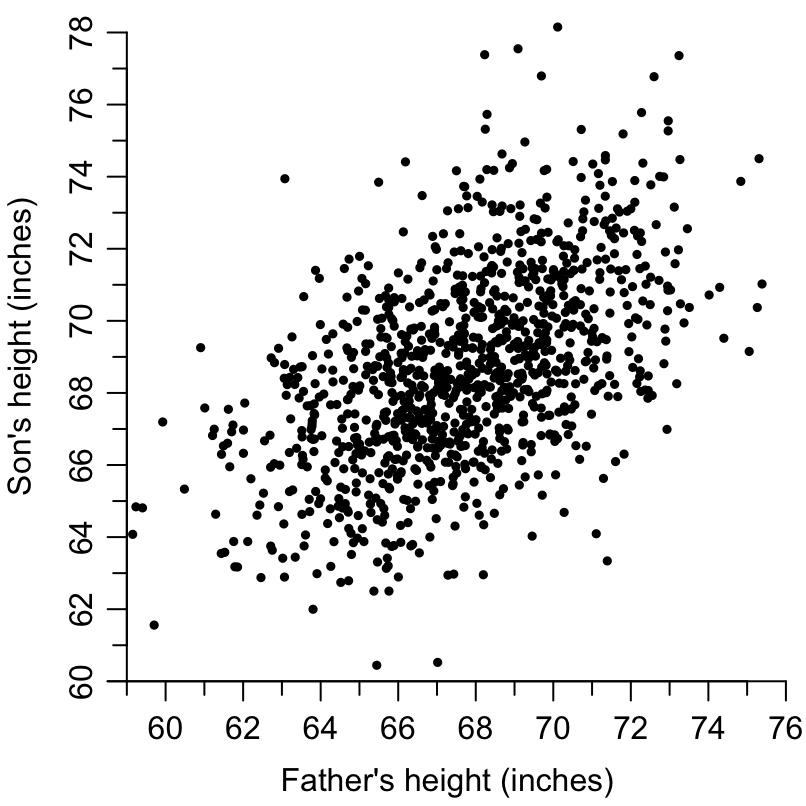
\includegraphics[width=0.63\linewidth]{ch10_24spr_files/figure-beamer/unnamed-chunk-1-1} \end{flushright}

\vspace{-2.5in}
\begin{minipage}{.35\textwidth}
\begin{itemize}
\item The plot shows a moderate linear relationship between fathers' heights and the sons' heights
\item For a father of a given height, what height would you predict for his son?
\end{itemize}
\end{minipage}
\end{frame}

\begin{frame}{The SD Line \& The Regression Line}
\protect\hypertarget{the-sd-line-the-regression-line}{}
\begin{flushright}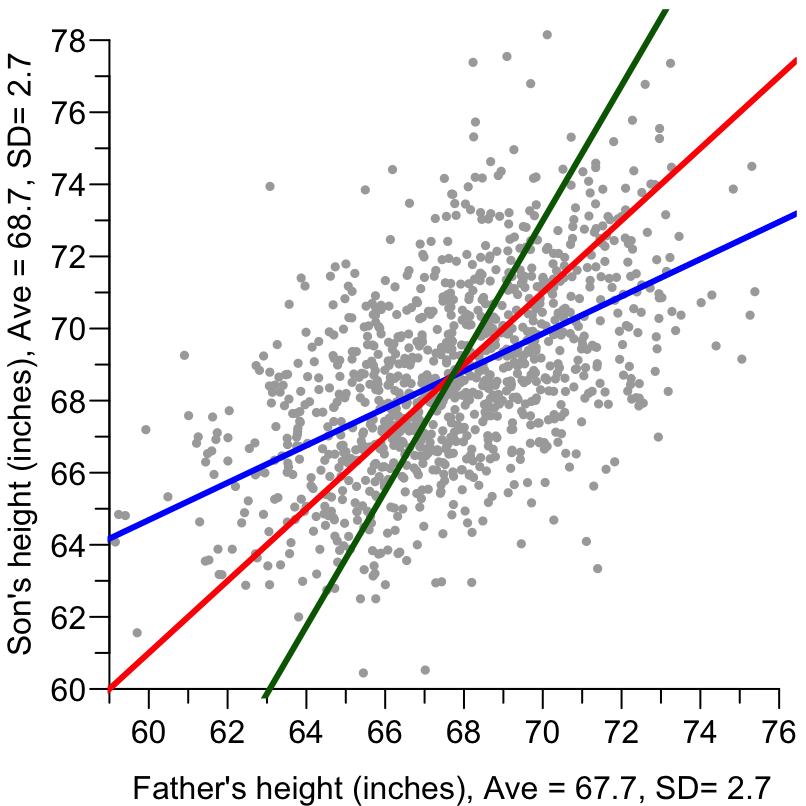
\includegraphics[width=0.63\linewidth]{ch10_24spr_files/figure-beamer/unnamed-chunk-2-1} \end{flushright}

\vspace{-2in}
\begin{minipage}{.35\textwidth}
\begin{itemize}
\item \textcolor{red}{Red}: the \red{SD line}.
\item \textcolor{blue}{Blue}: the \red{regression line} to predict the son's height from from his father's height
\item We will introduce the \textcolor{green}{Green} line shortly.
\end{itemize}
\end{minipage}
\medskip

Which line do you think is the best to predict son's height from
father's height?
\end{frame}

\begin{frame}{The SD Line}
\protect\hypertarget{the-sd-line}{}
\begin{itemize}
\tightlist
\item
  The SD line goes through the point of averages \((\bar{x},\bar{y})\).
\item
  When
  \(\displaystyle{ \begin{array}{c} r > 0\\[-3pt] r < 0 \end{array}}\) ,
  the line
  \(\displaystyle{ \begin{array}{c} \text{rises}\\[-3pt] \text{falls} \end{array}}\)
  one vertical SD for each run of one horizontal SD.
\item
  The SD line is about the same as the long axis of the oval which
  encircle the main portion of the cloud of points.
\end{itemize}

\begin{center}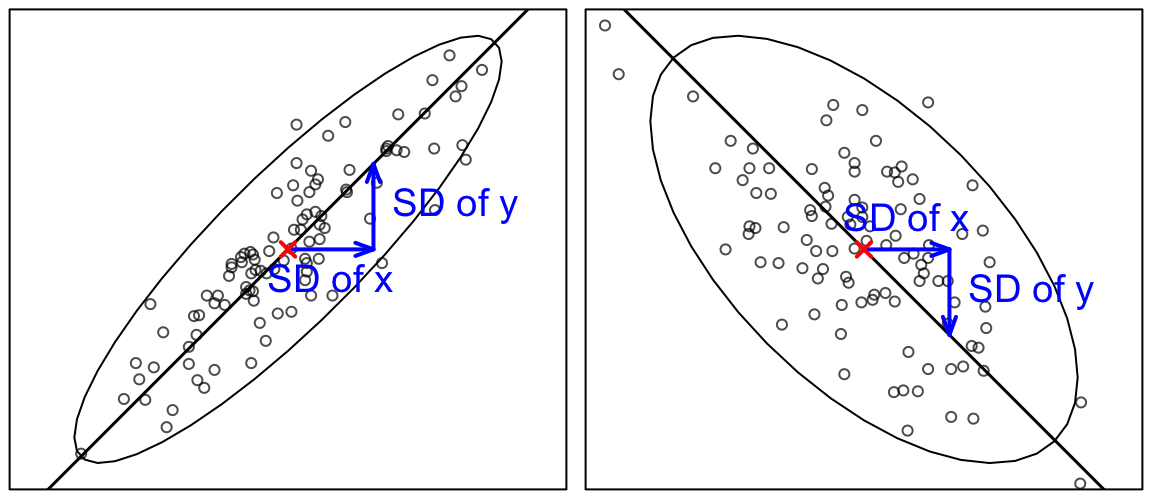
\includegraphics[width=0.95\linewidth]{ch10_24spr_files/figure-beamer/unnamed-chunk-3-1} \end{center}
\end{frame}

\begin{frame}{Regression Line v.s. SD Line}
\protect\hypertarget{regression-line-v.s.-sd-line}{}
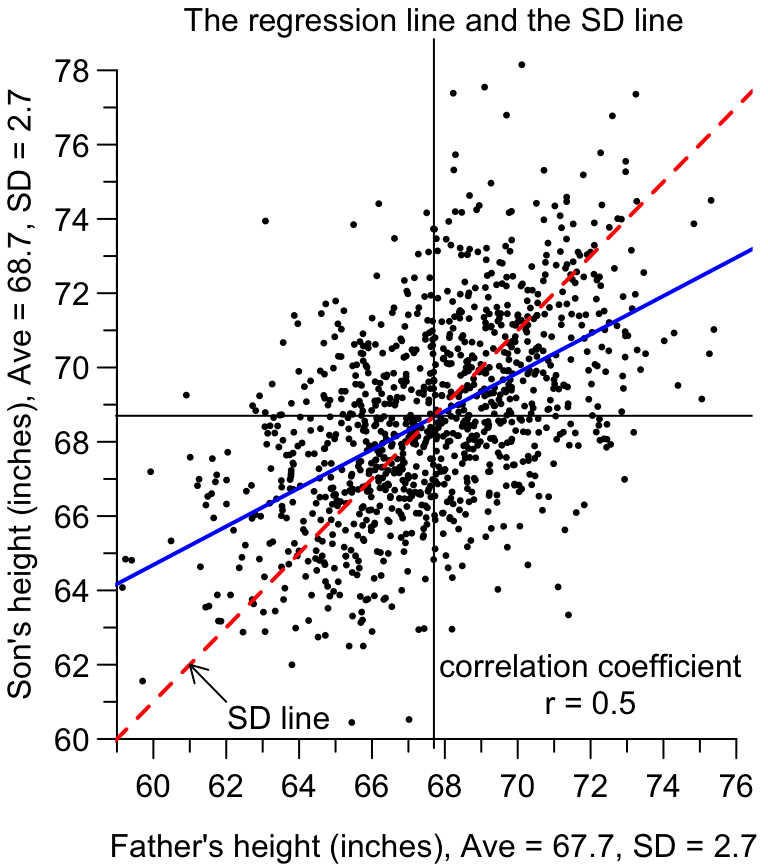
\includegraphics[width=0.5\linewidth]{ch10_24spr_files/figure-beamer/unnamed-chunk-4-1}
\vspace{-2.5in}

\begin{flushright}
\begin{minipage}{0.55\textwidth}
\begin{itemize}
\item Both lines go through the point of averages $(\bar{x},\bar{y})$.

\item The regression line is \red{less steeply sloped} than the SD line, by a factor of $r$.

\item If $r>0$, whenever $X$ increases by 1 (SD of $X$), $Y$ only
increase of only $r$ (SD of $Y$)
\item If $r<0$, whenever $X$ increases by 1 (SD of $X$), $Y$ only
decrease of only $r$ (SD of $Y$)
\end{itemize}
\end{minipage}
\end{flushright}
\end{frame}

\begin{frame}{}
\protect\hypertarget{section}{}
The points in the vertical chimney are the father-son pairs where the
father is \only<1-2>{72}\only<3>{70}\only<4->{64} inches tall, to the
nearest inch.

\only<1| handout:0>{


\begin{center}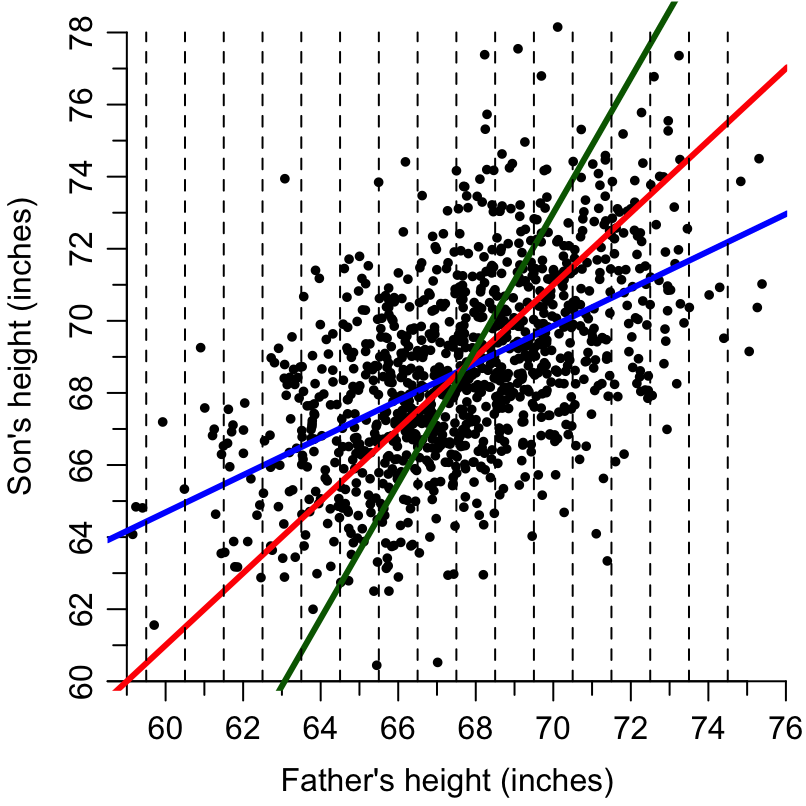
\includegraphics[width=0.63\linewidth]{ch10_24spr_files/figure-beamer/unnamed-chunk-5-1} \end{center}


}\only<2| handout:0>{


\begin{center}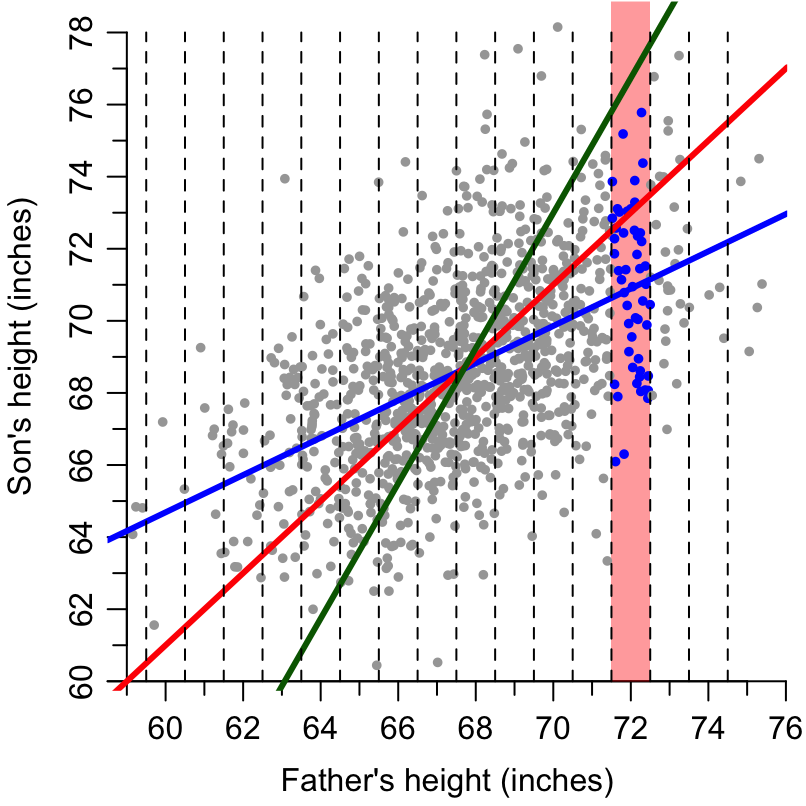
\includegraphics[width=0.63\linewidth]{ch10_24spr_files/figure-beamer/unnamed-chunk-5-2} \end{center}


}\only<3| handout:0>{


\begin{center}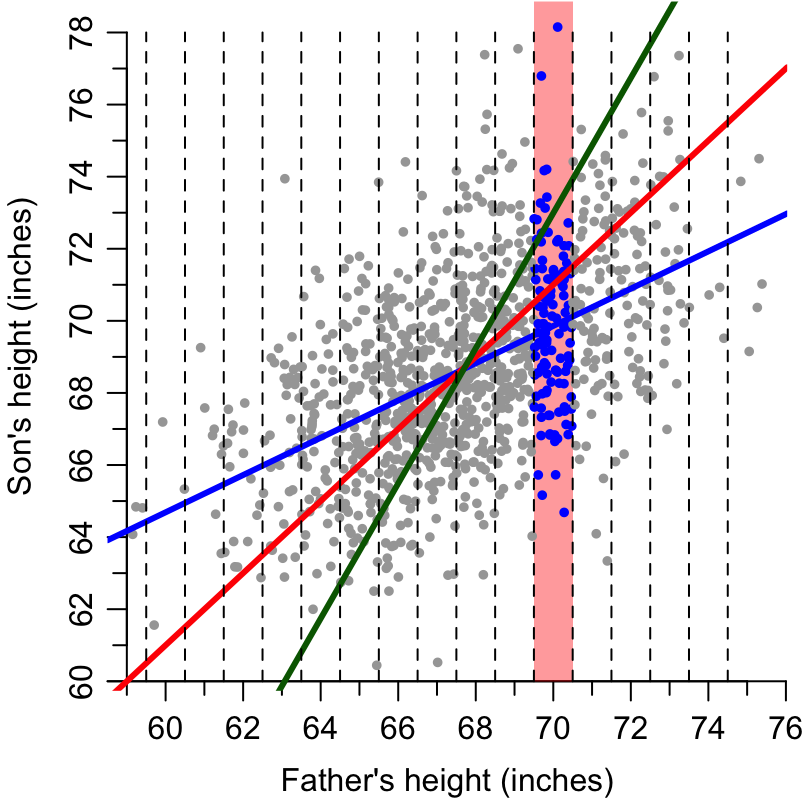
\includegraphics[width=0.63\linewidth]{ch10_24spr_files/figure-beamer/unnamed-chunk-5-3} \end{center}


}\only<4| handout:0>{


\begin{center}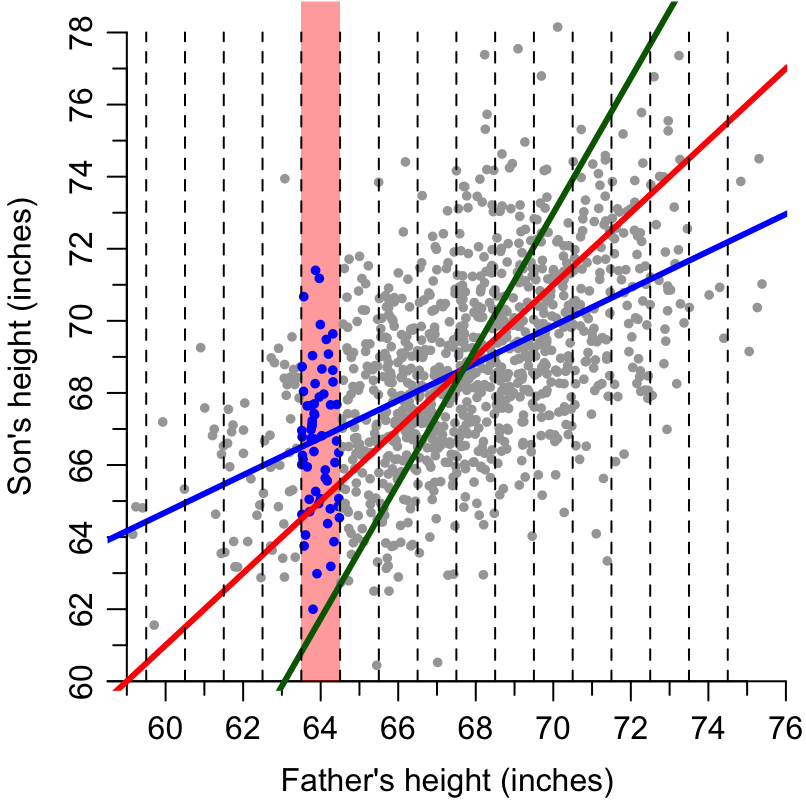
\includegraphics[width=0.63\linewidth]{ch10_24spr_files/figure-beamer/unnamed-chunk-5-4} \end{center}


}\only<5| handout:1>{


\begin{center}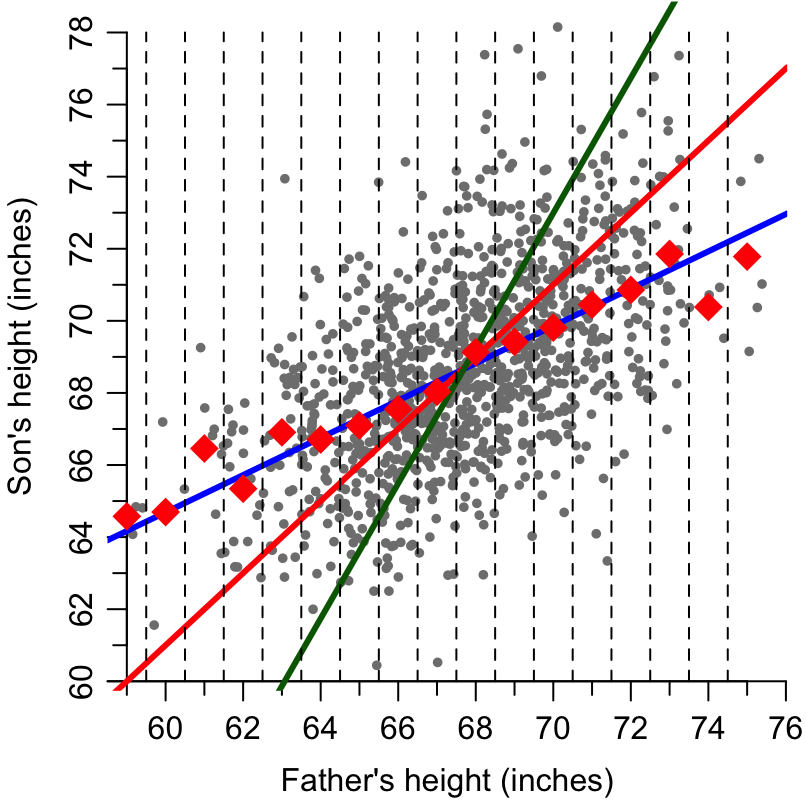
\includegraphics[width=0.63\linewidth]{ch10_24spr_files/figure-beamer/unnamed-chunk-5-5} \end{center}


}
\end{frame}

\begin{frame}{Why the Regression Line \(\neq\) the SD line?}
\protect\hypertarget{why-the-regression-line-neq-the-sd-line}{}
For a football-shaped scatter diagram, as the football is cut into
vertical strips, the midpoints of the vertical strips falls on the
regression line, not the SD line

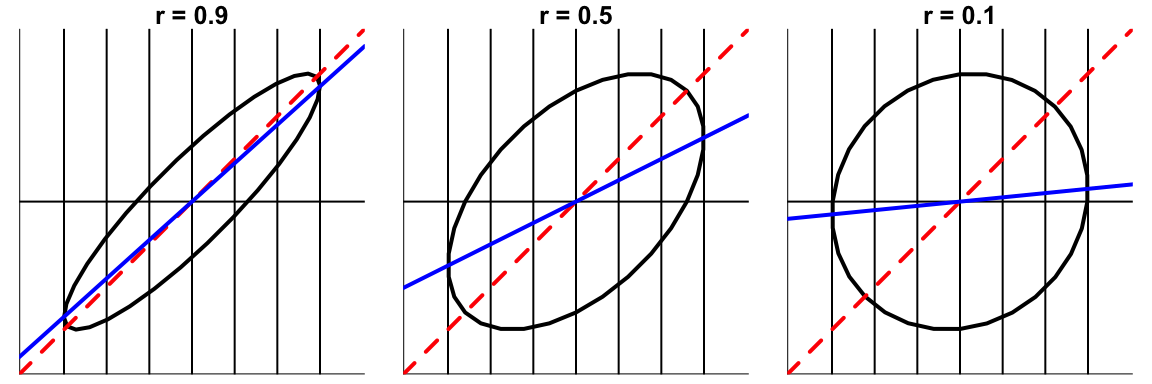
\includegraphics[width=1\linewidth]{ch10_24spr_files/figure-beamer/unnamed-chunk-6-1}

\begin{itemize}
\tightlist
\item
  SD line is used to describe the shape of the scatter diagram, not for
  prediction.
\item
  When \(r=1\) or \(r=-1\), the two lines coincide.
\end{itemize}
\end{frame}

\begin{frame}{Where Does the Term ``Regression'' Come From?}
\protect\hypertarget{where-does-the-term-regression-come-from}{}
\vspace{-8pt}

Sons of fathers who are
\(\displaystyle{ \begin{array}{l} \text{taller}\\[-3pt] \text{shorter} \end{array} }\)
than average are themselves
\(\displaystyle{ \begin{array}{l} \text{taller}\\[-3pt] \text{shorter} \end{array} }\)
than average, but by not so much as the fathers. \medskip

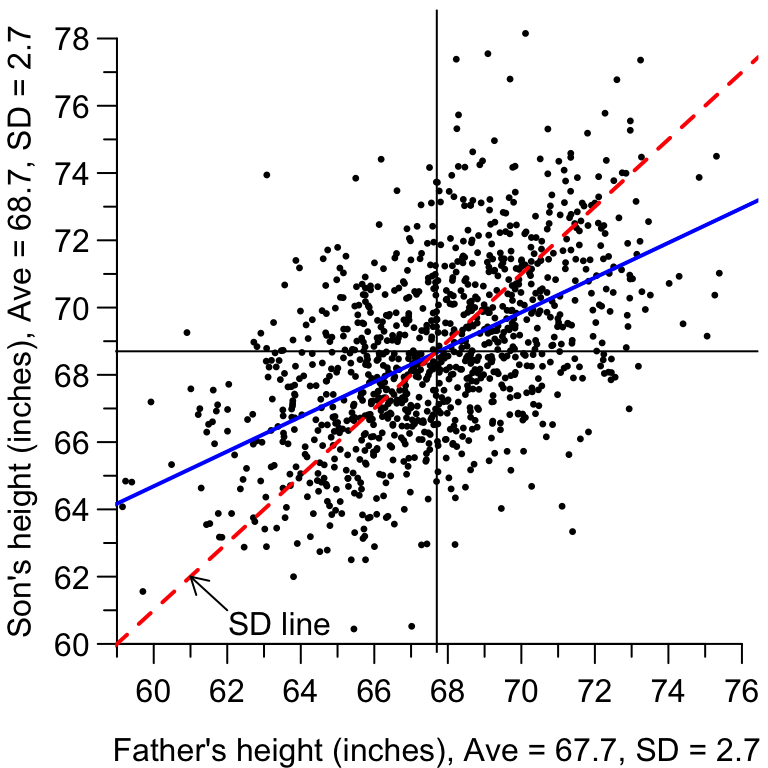
\includegraphics[width=0.5\linewidth]{ch10_24spr_files/figure-beamer/unnamed-chunk-7-1}
\vspace{-2.3in}

\begin{flushright}
\begin{minipage}{.5\textwidth}
\begin{itemize}
\item  There is a "falling back"towards the mean.
In Galton's terms:
a regression towards mediocrity."\medskip

\item  The term "regression" is widely used in statistics
in connection with how one variable varies with respect to another.
\end{itemize}
\end{minipage}
\end{flushright}
\end{frame}

\begin{frame}{}
\protect\hypertarget{section-1}{}
\textbf{Q}: Why do sons of fathers who are taller than average tend
themselves to be taller than average, but by not so much as their
fathers? \pause

\begin{itemize}
\item
  Their mothers might not be as exceptionally tall as their
  fathers.\pause \bigskip\bigskip
\item
  Diet, exercise, and other environmental factors also influence height.
  It is more common to get an average level of diet, exercise, and other
  factors than to get exceptional level of these factors.
\end{itemize}
\end{frame}

\begin{frame}{The Regression Method}
\protect\hypertarget{the-regression-method}{}
\vspace{-16pt}
\begin{minipage}{.75\textwidth}
For any football-shaped scatterplot (i.e., the
majority of the points in the plot are distributed in
a sloped oval), the average value of $y$ corresponding to
a given value of $x$ may be estimated by the regression
line (for $y$ on $x$).
\vspace{-1.2in}
\end{minipage}

\begin{flushright}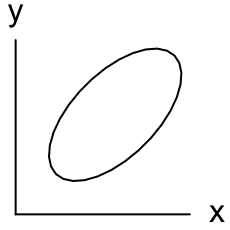
\includegraphics[width=0.2\linewidth]{ch10_24spr_files/figure-beamer/unnamed-chunk-8-1} \end{flushright}

\begin{flushleft}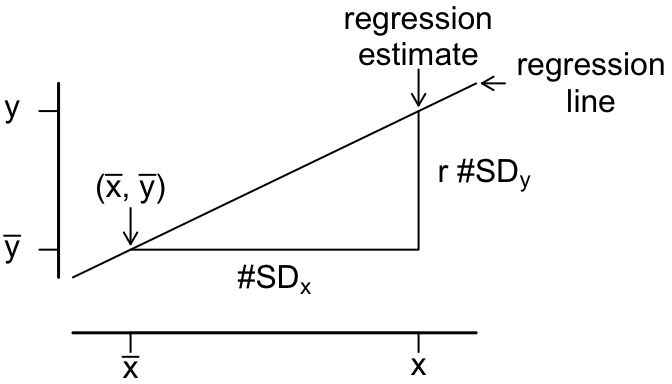
\includegraphics[width=0.6\linewidth]{ch10_24spr_files/figure-beamer/unnamed-chunk-9-1} \end{flushleft}
\vspace{-1.2in}
\begin{flushright}
\begin{minipage}{.48\textwidth}
For however many SDs $x$ is above or below $\bar{x}$,\\
the regression estimate for \textbf{the conditional average of $y$ given $x$}
is only $r$ times that many SDs above or below $\bar{y}$.
\end{minipage}
\end{flushright}

\medskip

Whenever \(x\) goes up by 1 SD\(_x\), \(y\) goes up by \(r\) SD\(_y\),
on average.
\end{frame}

\begin{frame}{Why is \(r\) the Right Factor?}
\protect\hypertarget{why-is-r-the-right-factor}{}
\underline{Short answer}: it just turns out that way.\newline It happens
that way for all football-shaped scatted diagrams, e.g.~Pearson's
father-son data. \medskip

\underline{Long answer}:\newline Three special cases are easy to
understand: \(r = 0\), 1, and \(-1\).

\begin{itemize}
\item
  If \(r=0\), there is no association between \(x\) and \(y\). For a one
  SD increase in \(x\), there is no increase or decrease in \(y\), on
  average.
\item
  If \(r=1\), there is a perfect positive association between \(x\) and
  \(y\). A one SD increase in \(x\) corresponds exactly to a one SD
  increase in \(y\).
\item
  If \(r=-1\), there is a perfect negative association. A one SD
  increase in \(x\) corresponds exactly to a one SD decrease in \(y\).
\end{itemize}
\end{frame}

\begin{frame}{Nonlinear Association}
\protect\hypertarget{nonlinear-association}{}
\begin{flushleft}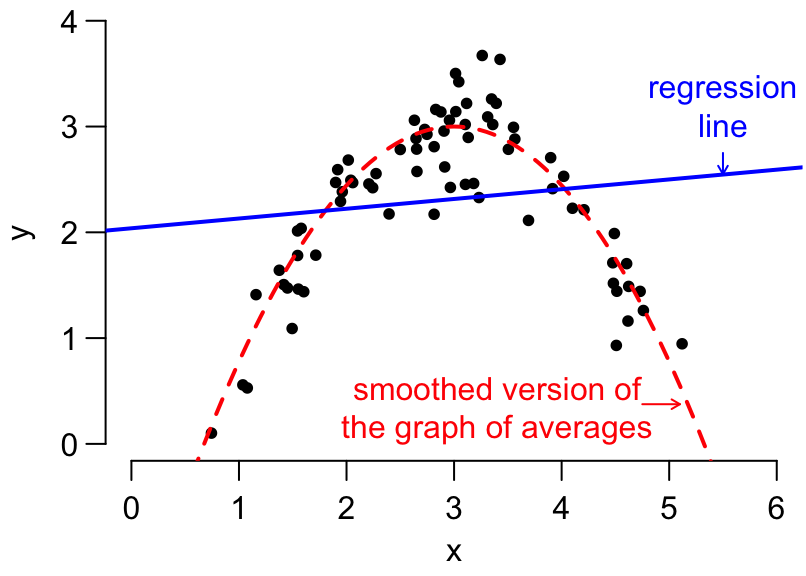
\includegraphics[width=0.55\linewidth]{ch10_24spr_files/figure-beamer/unnamed-chunk-10-1} \end{flushleft}
\vspace{-2in}
\begin{flushright}
\begin{minipage}{.47\textwidth}
\begin{itemize}
\item \textbf{Beware}: linear regression doesn't make sense when the data structure isn't linear.
\item You can always use the graph of averages to describe how $y$ changes with respect to $x$, on average.
\end{itemize}
\end{minipage}
\end{flushright}

\begin{itemize}
\tightlist
\item
  It usually makes sense to smooth the graph of averages to get a
  simpler description of the variation.
\item
  But when the pattern in the data is nonlinear, it doesn't make sense
  to smooth the graph of averages to a straight line.

  \begin{itemize}
  \tightlist
  \item
    How do you tell if pattern in the data is nonlinear?
  \end{itemize}
\end{itemize}
\end{frame}

\begin{frame}{Predictions for Individuals}
\protect\hypertarget{predictions-for-individuals}{}
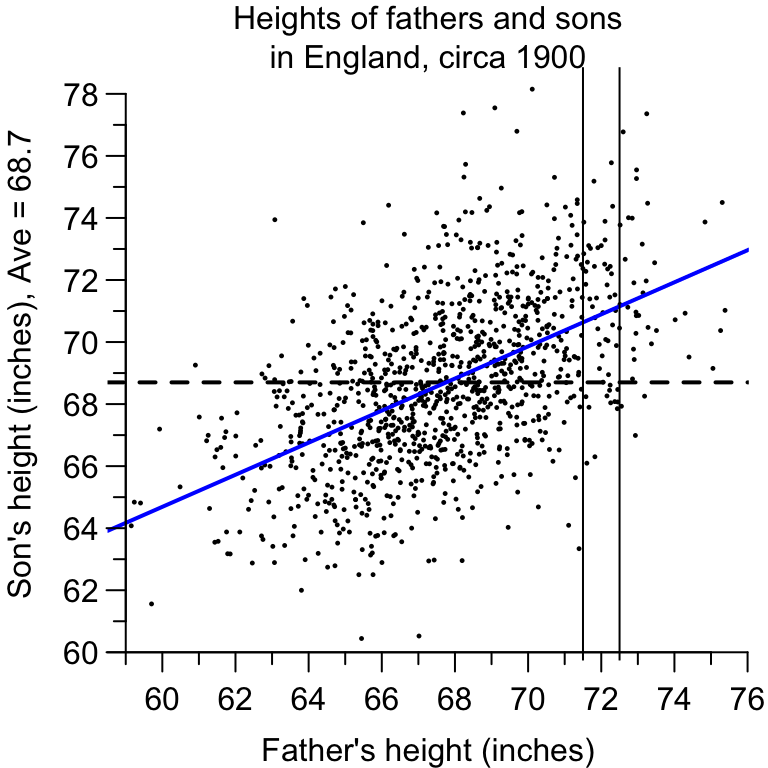
\includegraphics[width=0.52\linewidth]{ch10_24spr_files/figure-beamer/FS6-1}
\vspace{-2.4in}

\begin{flushright}
\begin{minipage}{.48\textwidth}
Consider again the 1,078 pairs of fathers and sons.
\medskip

I'm going to pick one of these pairs at random, and ask you to predict the son's height.
\begin{itemize}
\item If I tell you nothing about the father, your prediction would be
 \Hide{2-}{68.7 inches}.
In the diagram, that corresponds to using the \Hide{2-}{horizontal dash} line.
\end{itemize}
\end{minipage}
\end{flushright}

\begin{itemize}
\tightlist
\item
  If I tell you the father's height, your prediction would be
  \hide{3-}{ave ht of sons w/ fathers of that ht}. In the diagram, that
  corresponds to using the \Hide{3-}{regression line}.
\end{itemize}
\end{frame}

\begin{frame}{Be Cautious for Extrapolation}
\protect\hypertarget{be-cautious-for-extrapolation}{}
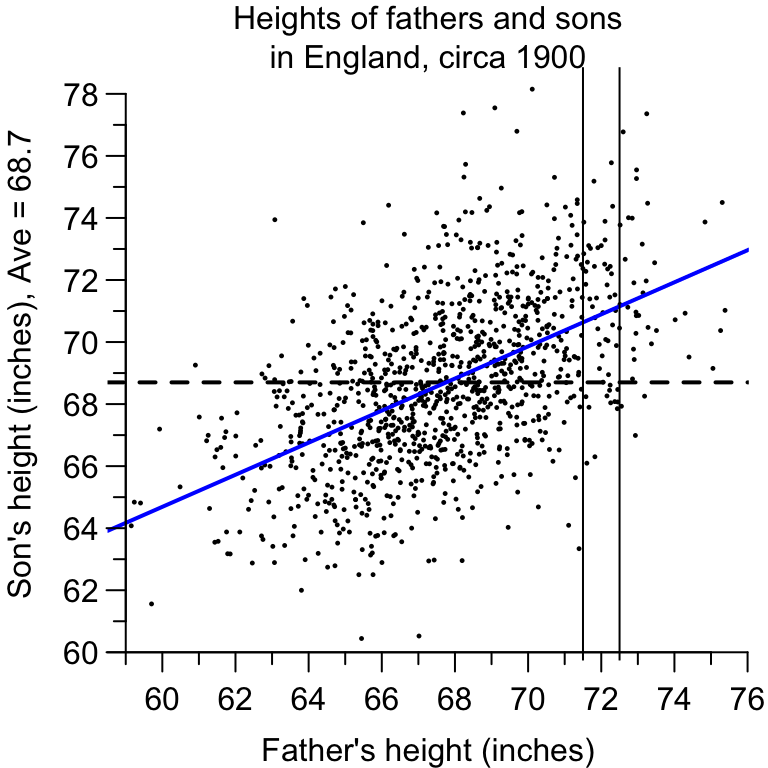
\includegraphics[width=0.52\linewidth]{ch10_24spr_files/figure-beamer/unnamed-chunk-11-1}
\vspace{-2.2in}

\begin{flushright}
\begin{minipage}{.48\textwidth}
Would you use the regression line to predict the height of a son:
\begin{itemize}
\item For fathers in England circa 1900?
\item For fathers in England circa 1900 who were extremely short/tall?
\item For fathers in the U.S. in 2011?
\end{itemize}
\end{minipage}
\end{flushright}
\vspace{20pt}

A regression line can be used to make predictions for individuals. But
if you have to extrapolate far from the data, or to a different group of
subjects, watch out!
\end{frame}

\begin{frame}{Using the Regression Line}
\protect\hypertarget{using-the-regression-line}{}
\newcommand\inch{{\tt "}}
\newcommand\foot{{\tt '}}

Consider the father-son data. The scatter plot is football-shaped.
\begin{align*}
\text{average height of fathers}&\approx68{\tt "},\;\text{SD}\approx 3{\tt "}\\
\text{average height of sons}   &\approx69{\tt "},\;\text{SD}\approx 3{\tt "},\;\; r\approx 0.5
\end{align*} On average, how tall are sons of 6 foot fathers?

\begin{itemize}
\tightlist
\item
  A 6 foot father is \Hide{2-}{4} inches above average in height.
\item
  That's \Hide{3-}{4/3} of an SD.
\item
  The average height of sons of 6 foot fathers is \Hide{3-}{above} the
  overall average by \Hide{4-}{$0.5\times4/3=2/3$} of an SD.
\item
  That's \Hide{5-}{2} inches.
\item
  So sons of 6 foot fathers are on average \Hide{6-}{$69+2=71$} inches
  tall.
\end{itemize}
\end{frame}

\begin{frame}{Using the Regression Line (Cont'd)}
\protect\hypertarget{using-the-regression-line-contd}{}
Below is a summary for the height and systolic blood pressure for the
men ages 18--24 in the HANES sample.

\begin{center}
\tabcolsep=4pt
\begin{tabular}{r@{$\,\approx\,$}lr@{$\,\approx\,$}lc}
average height&68{\tt "},&SD&3{\tt "}\\[-3pt]
average blood pressure&124mm,&SD&15mm,& $r\approx -0.2$
\end{tabular}
\end{center}

The scatter diagram is football-shaped. Estimate the average blood
pressure of 64-inch tall men.\small

\textbf{Step 1}. Convert \(x=64\) into standard units:
\(\hid{2-}{(\text{SU of }x) =(64-68)/3=-4/3}\)\newline \textbf{Step 2}.
Multiply the SU in Step 1 by \(r=-0.2\). The product is the predicted
\(y\)-value in standard units.
\[\hid{3-}{r\times (\text{SU of }x) =(-0.2)\times(\dfrac{-4}{3})=\dfrac{4}{15}=(\text{SU of }y)}\]
\textbf{Step 3}. Convert the standard unit of the predicted \(y\)
\(\text{SU}_y\) back to the original scale.
\[\hid{4-}{\text{predicted }y=(\text{Ave of }y)+ (\text{SU of }y)(\text{SD of }y)=124+(4/15)\times 15\approx 128.}\]
So the average blood pressure of these men is estimated as
\Hide{5-}{128} mm.
\end{frame}

\begin{frame}{}
\protect\hypertarget{section-2}{}
In general, to predict the value of of \(y\) for a given value of \(x\),
you:

\par
\smallskip

\begin{enumerate}
[(1)]
\tightlist
\item
  convert the given value of \(x\) to \textbf{standard units},

  \par\smallskip
\item
  multiply by the \textbf{correlation ($r$)}, which gives the
  corresponding average value of \(y\) in standard units.

  \par\smallskip
\item
  convert back from standard units.
\end{enumerate}

\begin{center}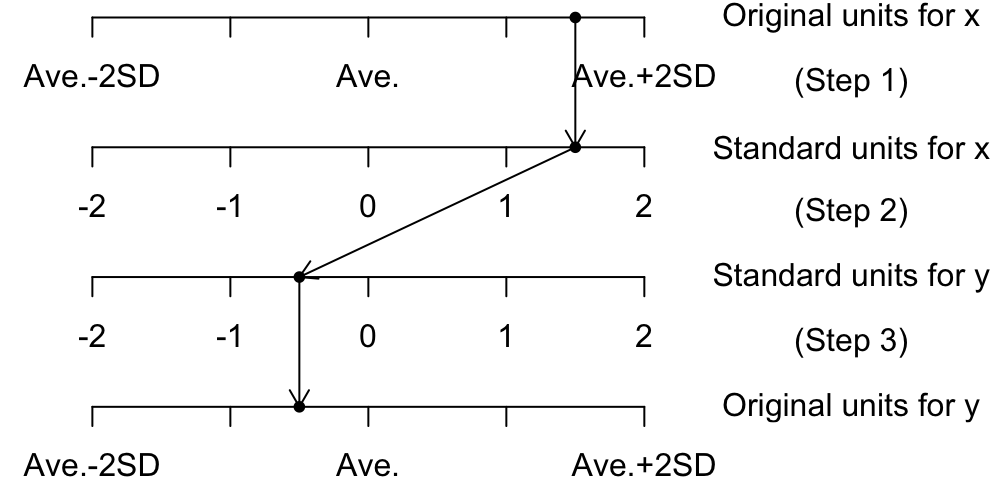
\includegraphics[width=0.8\linewidth]{ch10_24spr_files/figure-beamer/unnamed-chunk-12-1} \end{center}

In Step 1, you use the Average and SD of \alert{$x$} .\newline In Step
3, you use the Average and SD of \alert{$y$} .
\end{frame}

\begin{frame}{In-Class Exercise}
\protect\hypertarget{in-class-exercise}{}
For the men age 18 and over in HANES5,

\begin{center}
\begin{tabular}{lll}
average height $\approx 69$ inches,  & SD $\approx 3$ inches \\
average weight $\approx 190$ lbs, & SD $\approx 42$ lbs, & $r= 0.41$\\
\end{tabular}
\end{center}

\begin{enumerate}
[a.]
\tightlist
\item
  Predict the weight of a 70.8-inch tall man.
\item
  Predict the weight of a 64.5-inch tall man. \vspace{2in}
\end{enumerate}
\end{frame}

\begin{frame}{Answer to Exercise}
\protect\hypertarget{answer-to-exercise}{}
\begin{center}
\begin{tabular}{lll}
average height $\approx 69$ inches,  & SD $\approx 3$ inches \\
average weight $\approx 190$ lbs, & SD $\approx 42$ lbs, & $r= 0.41$\\
\end{tabular}
\end{center}

\vspace{-12pt}

\begin{enumerate}
[a.]
\tightlist
\item
  Predict the weight of a 70.8-inch tall man.
\end{enumerate}

\small

\begin{itemize}
\tightlist
\item
  Step 1. Convert \(x=70.8\) into standard units:
  \[(\text{SU of }x) =\dfrac{70.8-69}{3}=0.6\]
\item
  Step 2. Multiply the SU in Step 1 by \(r=0.41\). The product is the
  predicted \(y\)-value in standard units.
  \[r\times (\text{SU of }x) =0.41\times0.6=0.246=(\text{SU of }y)\]
\item
  Step 3. Convert the standard unit of the predicted \(y\) back to the
  original scale.
  \[ \text{predicted }y=(\text{Ave of }y)+ (\text{SU of }y)(\text{SD of }y)=190+0.246\times 42\approx 200.33.\]
  So 70.8-inch men on average weigh 200.33 lbs.
\end{itemize}
\end{frame}

\begin{frame}{Answer to Exercise}
\protect\hypertarget{answer-to-exercise-1}{}
\begin{center}
\begin{tabular}{lll}
average height $\approx 69$ inches,  & SD $\approx 3$ inches \\
average weight $\approx 190$ lbs, & SD $\approx 42$ lbs, & $r= 0.41$\\
\end{tabular}
\end{center}

\vspace{-12pt}

\begin{enumerate}
[a.]
\setcounter{enumi}{1}
\tightlist
\item
  Predict the weight of a 64.5-inch tall man.
\end{enumerate}

\small

\begin{itemize}
\tightlist
\item
  Step 1. Convert \(x=64.5\) into standard units:
  \[(\text{SU of }x) =\dfrac{64.5-69}{3}=-1.5\]
\item
  Step 2. Multiply the SU in Step 1 by \(r=0.41\). The product is the
  predicted \(y\)-value in standard units.
  \[r\times (\text{SU of }x) =0.41\times(-1.5)=-0.615=(\text{SU of }y).\]
\item
  Step 3. Convert the standard unit of the predicted \(y\) back to the
  original scale.
  \[\text{predicted }y=(\text{Ave of }y)+ (\text{SU of }y)(\text{SD of }y)=190+(-0.615)\times 42=164.17.\]
  So 64.5-inch men on average weigh 164.17 lbs.
\end{itemize}
\end{frame}

\hypertarget{test-retest-scenarioregression-effect-and-regression-fallacy}{%
\section{\texorpdfstring{Test-Retest Scenario,\newline Regression
Effect, and \newline Regression
Fallacy}{Test-Retest Scenario,Regression Effect, and Regression Fallacy}}\label{test-retest-scenarioregression-effect-and-regression-fallacy}}

\begin{frame}{The Test-Retest Scenario}
\protect\hypertarget{the-test-retest-scenario}{}
Each pitcher in a baseball team made one throw, the coach commented on
his performance before he made another throw.

\begin{flushleft}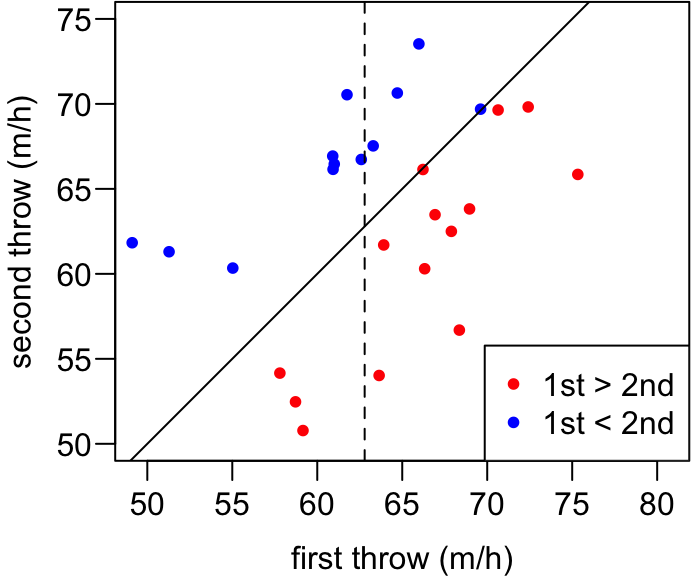
\includegraphics[width=0.5\linewidth]{ch10_24spr_files/figure-beamer/unnamed-chunk-13-1} \end{flushleft}
\vspace{-2in}
\begin{flushright}
\begin{minipage}{0.5\textwidth}
\begin{itemize}
\item vertical dash line marks the average of the 1st throw
\item Those who did above average in the first throw tended to do worse the second time (most points to the right of the vertical dash line are red)
\end{itemize}
\end{minipage}
\end{flushright}

\begin{itemize}
\tightlist
\item
  Conversely, those who performed below the average in the first throw
  mostly did better the second time (most points to the left of the
  vertical dash line are blue)
\item
  Does criticism help the pitchers while praise spoils them?
\end{itemize}
\end{frame}

\begin{frame}{The Regression Effect and the Regression Fallacy}
\protect\hypertarget{the-regression-effect-and-the-regression-fallacy}{}
\begin{itemize}
\item
  In a typical test-retest situation, the subjects get different scores
  on the two tests. Take the bottom group on the first test. Some
  improve on the second test, others do worse; but on the average the
  bottom group shows an improvement. Now the top group. Some do better
  the second time, others fall back; but on average the top group does
  worse the second time. This is the \textbf{regression effect}, and it
  happens whenever the scatter diagram spreads out around the SD line
  into a football-shaped cloud of points.
\item
  The \textbf{regression fallacy} consists in thinking that the
  regression effect is due to something other than spread around the SD
  line.
\end{itemize}
\end{frame}

\begin{frame}{Example: Sports Illustrated Cover Jinx}
\protect\hypertarget{example-sports-illustrated-cover-jinx}{}
\begin{columns}[T]
\begin{column}{.5\textwidth}
\parbox[m]{\textwidth}{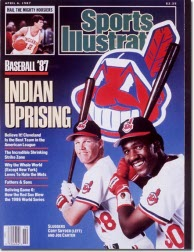
\includegraphics[width=1.05\textwidth]{./C10/SportsIllustrated1987.jpg}}
{\small \linespread{0.9} The April 6, 1987 \textit{Sports Illustrated} ``Indian Uprising'' cover.}
\end{column}
\begin{column}{.5\textwidth}
\textit{Individuals or teams who appear on the cover of the Sports Illustrated magazine will subsequently be jinxed.}

\bigskip
In 1987, the Indians won 61 and lose 101 games, the worst of any team that season.
\bigskip

Not due to the jinx, but the regression effect.
\end{column}
\end{columns}
\end{frame}

\hypertarget{there-are-two-regression-lines}{%
\section{There Are Two Regression
Lines}\label{there-are-two-regression-lines}}

\begin{frame}{}
\protect\hypertarget{section-3}{}
On p.16, we predicted that sons of 72-inch tall fathers are on average
71-inch tall. \textbf{True or False}: fathers of 71-inch tall sons are
on average 72-inch tall.

\begin{flushright}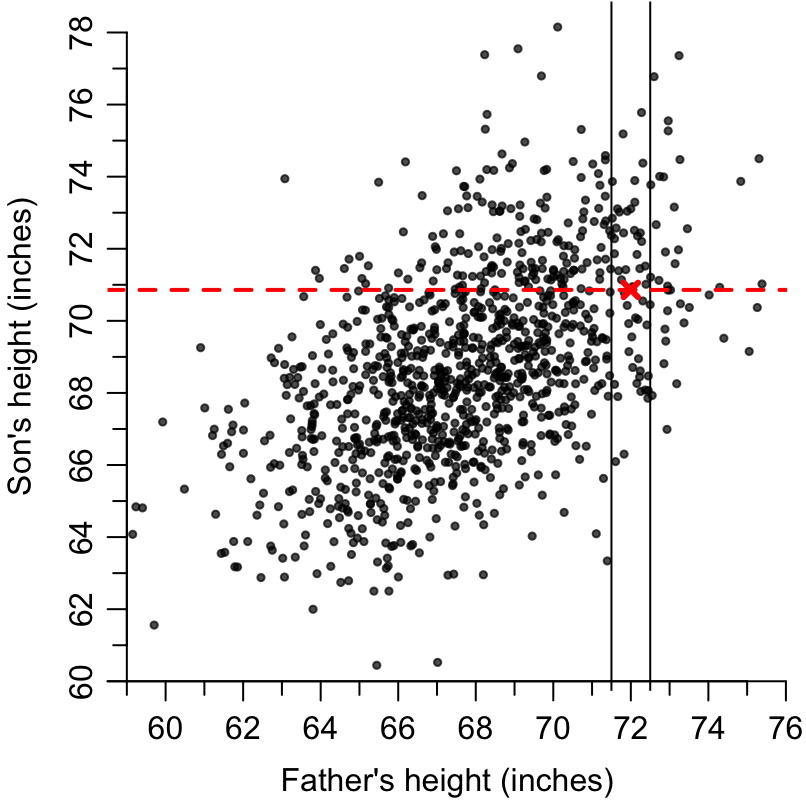
\includegraphics[width=0.72\linewidth]{ch10_24spr_files/figure-beamer/unnamed-chunk-14-1} \end{flushright}
\end{frame}

\begin{frame}{There Are Two Regression Lines}
\protect\hypertarget{there-are-two-regression-lines-1}{}
As well as regressing SH on FH, we can also regress FH on SH:

\begin{flushleft}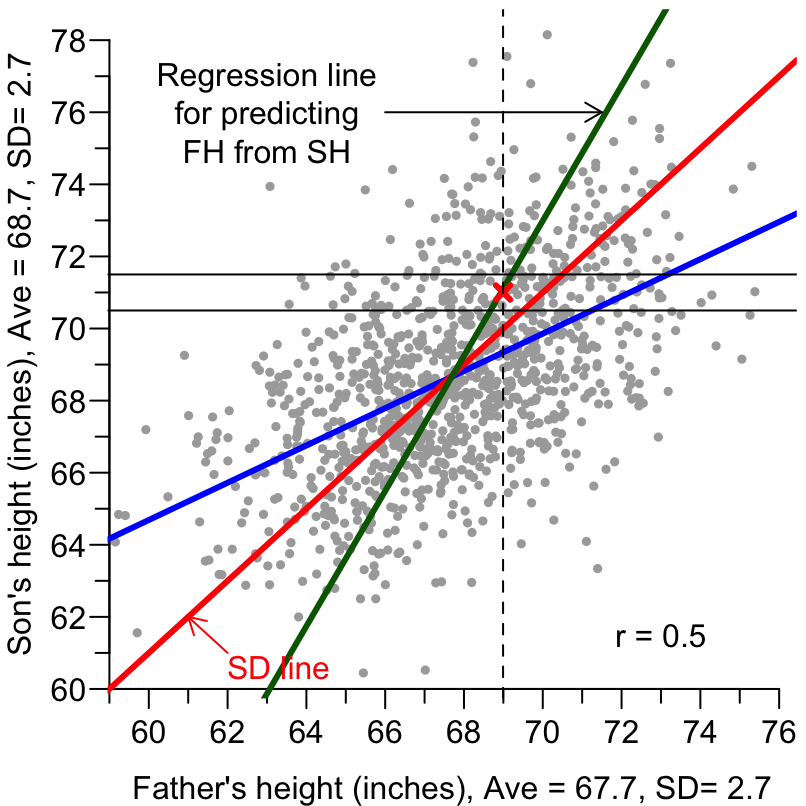
\includegraphics[width=0.54\linewidth]{ch10_24spr_files/figure-beamer/unnamed-chunk-15-1} \end{flushleft}

\vspace{-2.5in}
\begin{flushright}
\begin{minipage}{.5\textwidth}
\begin{itemize}
\item Points in the horizontal strip are the father-son pairs where
the son is 71{\tt "}~ tall, to the nearest inch.
\item The cross at the point $(68.99, 71)$ marks the average height
of the fathers of these sons.
The cross lies very close to the regression line for FH
on SH, which predicts these fathers to be only  \Hide{2-}{68.99{\tt "}}, not 72{\tt "}.
\end{itemize}
\end{minipage}
\end{flushright}
\end{frame}

\begin{frame}{Comparison of the Two Regression Lines}
\protect\hypertarget{comparison-of-the-two-regression-lines}{}
\begin{center}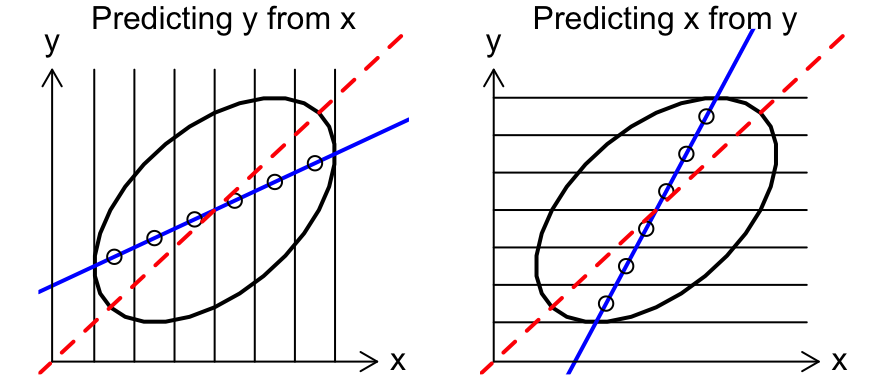
\includegraphics[width=0.75\linewidth]{ch10_24spr_files/figure-beamer/unnamed-chunk-16-1} \end{center}
\linespread{.9}

The regression line for predicting
\(\begin{array}{c} \textcolor{red}{\text{$y$ from $x$}} \\[-3pt] \textcolor{blue}{\text{$x$ from $y$}} \end{array}\)
involves:

\vspace{-10pt}

\begin{itemize}
\tightlist
\item
  dividing the scatter diagram into
  \(\begin{array}{c} \textcolor{red}{\text{vertical}}\\[-3pt] \textcolor{blue}{\text{horizontal}} \end{array}\)
  strips; \vspace{-6pt}
\item
  finding the average value of
  \(\begin{array}{c}\textcolor{red}{y}\\[-3pt] \textcolor{blue}{x}\end{array}\)
  in each strip; and
\item
  smoothing the resulting graph of averages to a straight line.
\end{itemize}

The line goes through the point of averages and is
\(\begin{array}{c} \textcolor{red}{\text{less}} \\[-3pt] \textcolor{blue}{\text{more}} \end{array}\)
steeply sloped than the SD line by a factor of
\(\begin{array}{c} \textcolor{red}{|r|}\\[-3pt] \textcolor{blue}{1/|r|} \end{array}\)
\end{frame}

\begin{frame}{There Are Two Regression Lines (Cont'd)}
\protect\hypertarget{there-are-two-regression-lines-contd}{}
Two regression lines can be drawn across a scatter diagram:

\begin{center}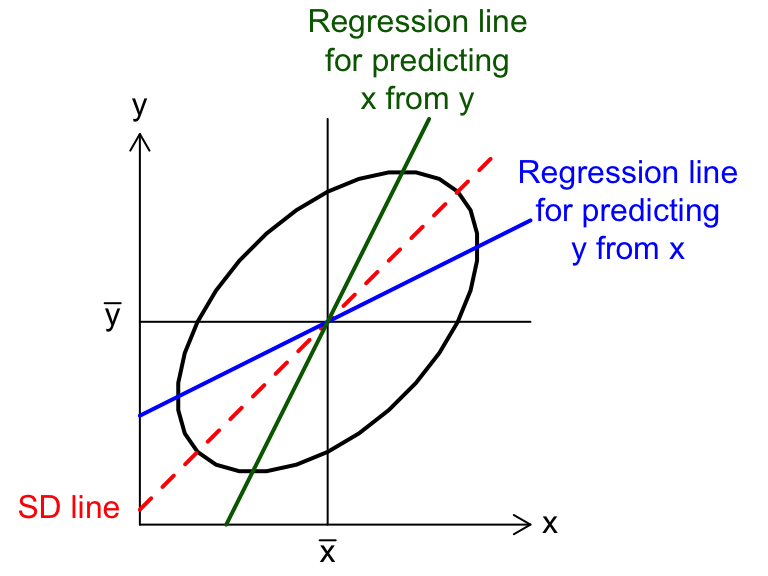
\includegraphics[width=0.65\linewidth]{ch10_24spr_files/figure-beamer/unnamed-chunk-17-1} \end{center}

In general the two regression lines are different. You can screw up a
prediction \textit{badly} by using the wrong line!

\begin{itemize}
\tightlist
\item
  When will the two lines be the same? \hid{2-}{When $r=1$ or $-1$.}
\end{itemize}
\end{frame}

\begin{frame}{Summary}
\protect\hypertarget{summary}{}
\begin{itemize}
\tightlist
\item
  Associated with each increase of one SD in \(x\) there is an increase
  of only \(r\) SDs in \(y\), on the average. Plotting these
  \textit{regression
  estimates} gives the \textit{regression line} of \(y\) on \(x\).
\item
  The \textit{graph of averages} is often close to a straight line, but
  may be a little bumpy. The regression line smooths out the bumps. If
  the graph of averages is a straight line, then it coincides with the
  regression line.
\item
  The regression line can be used to make predictions of one variable
  from another. But if you have to extrapolate far from the data, or to
  a different group of subjects, be careful.
\item
  Beware of nonlinear structure and outliers. They can fool the
  regression method.
\item
  Remember the regression effect and the regression fallacy.
\item
  You can draw two different regression lines on a scatter diagram: one
  predicts \(y\) from \(x\); the other predicts \(x\) from \(y\).
\end{itemize}
\end{frame}

\end{document}
